\section{Resultados}

	\subsection{Error de los autovectores calculados}
		
		Calculando el error de los autovectores obtenidos mediante el m\'etodo
		de la potencia\footnote{De la manera que se explica en el \textbf{Desarrollo}.}
		bajo distintos niveles de tolerancia obtenemos el siguiente resultado:

		\vspace{5mm}
		\centerline{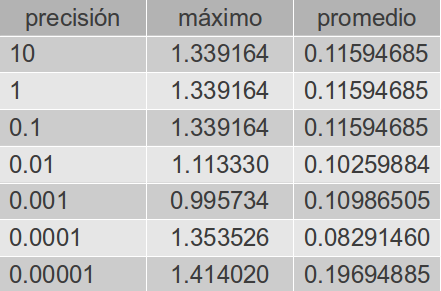
\includegraphics[width=7cm]{img/maxMed.png}}
		\centerline{\textsc{Tolerancia Vs error m\'aximo y error promedio de los autovectores}}
		\centerline{M\'etodo de la potencia en instancia \texttt{primeros5000.dat}}
		\vspace{5mm}

		Vemos que los resultados mejoran hasta la tolerancia de $0.001$, luego se
		desestabilizan.

		Cuando realizamos este mismo test al m\'etodo \textit{QR-potencia Inversa}
		no obtuvimos resultados significativos. Es decir, para toda tolerancia el
		error es de a lo sumo $10^{-5}$ y por lo tanto no nos result\'o significativo.

	\subsection{Diferencias en el tiempo de ejecuci\'on para obtener autovectores}

		Comparamos el tiempo de ejecuci\'on de ambas estrategias con distintas tolerancias entre $10$ y 
		$10^{-6}$, para esto calculamos el promediando de la cantidad de ticks que tardaba cada una en 
		finalizar durante diez corridas\footnote{ Ver Tabla A }.

	 	\vspace{5mm}
		\centerline{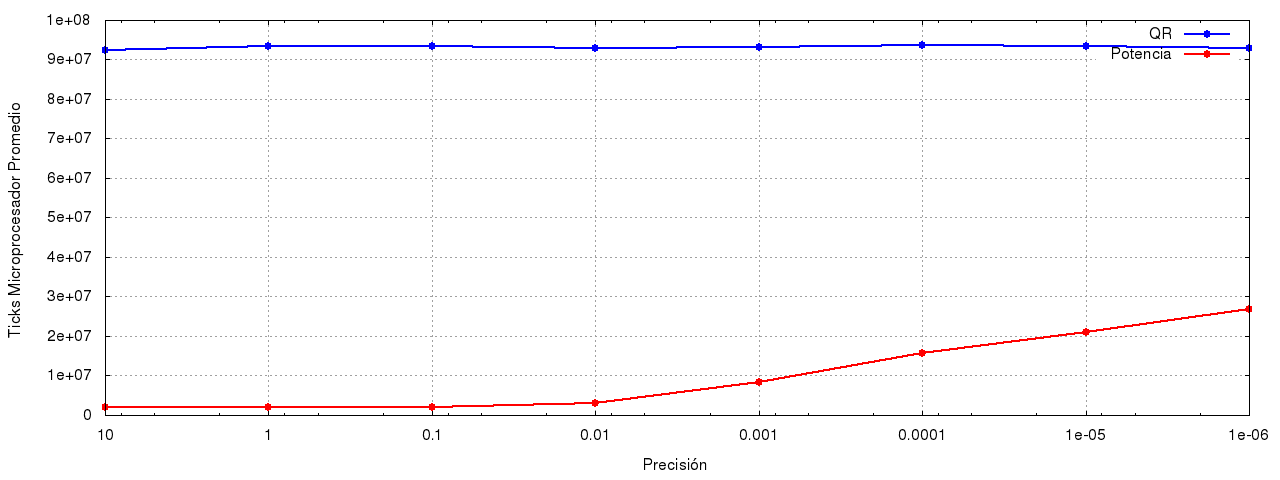
\includegraphics[width=20cm]{img/precVsTick.png}}
		\centerline{\textsc{Tolerancia Vs Cantidad de ciclos de procesador}}
		\centerline{M\'etodo de la potencia y m\'etodo \textit{QR-potencia Inversa} en instancia
		\texttt{primeros5000.dat}}
		\vspace{5mm}


	\subsection{Cantidad de d\'igitos reconocidos en funci\'on del m\'etodo,
	cantidad de componentes utilizada y la precisi\'on de los autovectores}

		Tomando una precisi\'on de $0.001$ buscamos la cantidad de vecinos que
		optimice el reconocimiento de d\'igitos.
		Para el m\'etodo de los vecinos ponderados obtenemos\footnote{ Ver Tabla B }:

		\vspace{5mm}
		\centerline{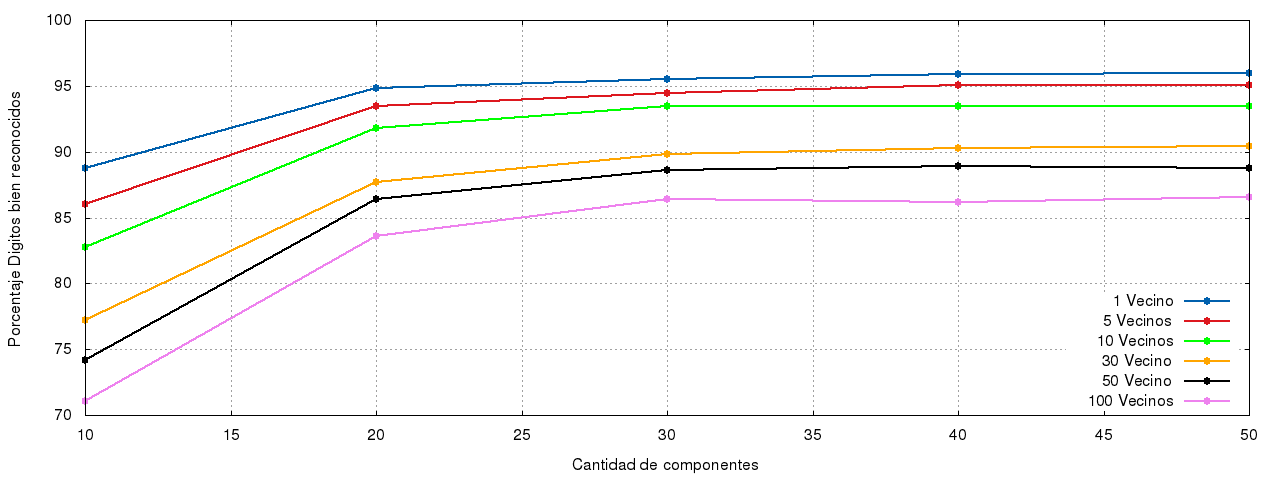
\includegraphics[width=20cm]{img/kPonderadosPS.png}}
		\centerline{\textsc{Cantidad de componentes Vs porcentaje de d\'igitos bien
		reconocidos}}
		\centerline{\textsc{variando cantidad de vecinos}}
		\centerline{M\'etodo de la potencia/$k$-vecinos-ponderados con tolerancia
		$0.001$ en instancia \texttt{primeros5000.dat}}
		\vspace{5mm}

		Para el m\'etodo est\'andar de los $k$-vecinos\footnote{ Ver Tabla C }:

		\vspace{5mm}
		\centerline{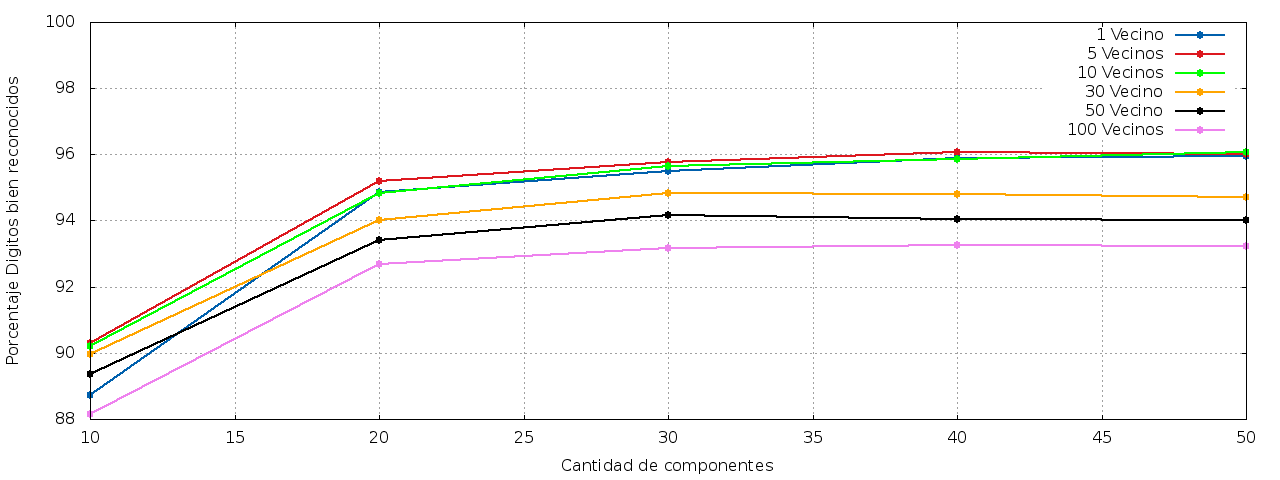
\includegraphics[width=20cm]{img/kVecinosPS.png}}
		\centerline{\textsc{Cantidad de componentes Vs porcentaje de d\'igitos bien
		reconocidos}}
		\centerline{\textsc{variando cantidad de vecinos}}
		\centerline{M\'etodo de la potencia/$k$-vecinos con tolerancia $0.001$ en instancia
		\texttt{primeros5000.dat}}
		\vspace{5mm}

		Una vez que encontramos una cantidad de vecinos adecuada comparamos los m\'etodos
		de c\'alculo de autovectores, variando la precisi\'on del m\'etodo de la potencia\footnote{ Ver Tabla D }:

		\vspace{5mm}
		\centerline{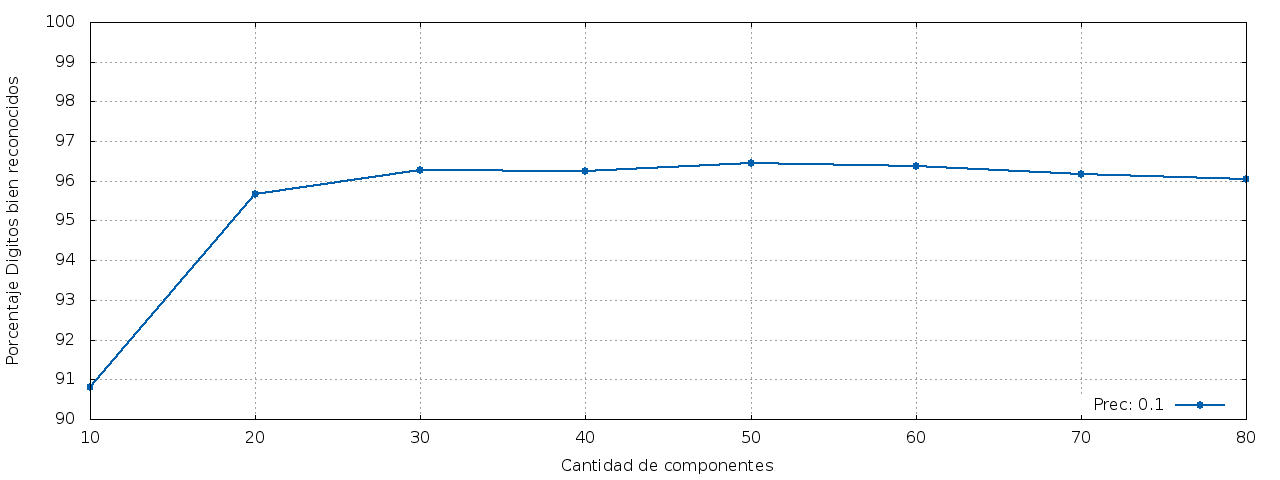
\includegraphics[width=20cm]{img/QRkVecinos.png}}
		\centerline{\textsc{Cantidad de componentes Vs porcentaje de d\'igitos bien
		reconocidos}}
		\centerline{M\'etodo \textit{QR-potencia Inversa}/$k$-vecinos con tolerancia $0.1$
		en instancia \texttt{primeros5000.dat}}
		\vspace{5mm}
		
		\vspace{5mm}
		\centerline{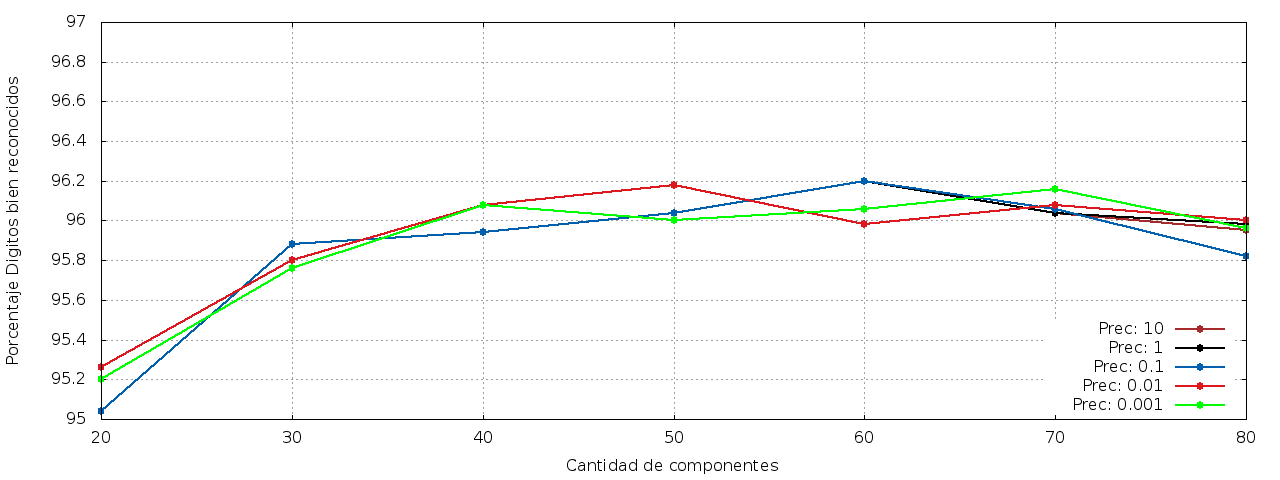
\includegraphics[width=20cm]{img/PSprec.png}}
		\centerline{\textsc{Cantidad de componentes Vs porcentaje de d\'igitos bien
		reconocidos}}
		\centerline{\textsc{variando la tolerancia}}
		\centerline{M\'etodo de la potencia/$k$-vecinos en instancia \texttt{primeros5000.dat}}
		\vspace{5mm}

		Finalmente comparamos con el comportamiento del m\'etodo de la distancia al promedio
		utilizando \textit{QR-potencia Inversa} para calcular autovectores\footnote{ Ver Tabla E }:
	
		\vspace{5mm}
		\centerline{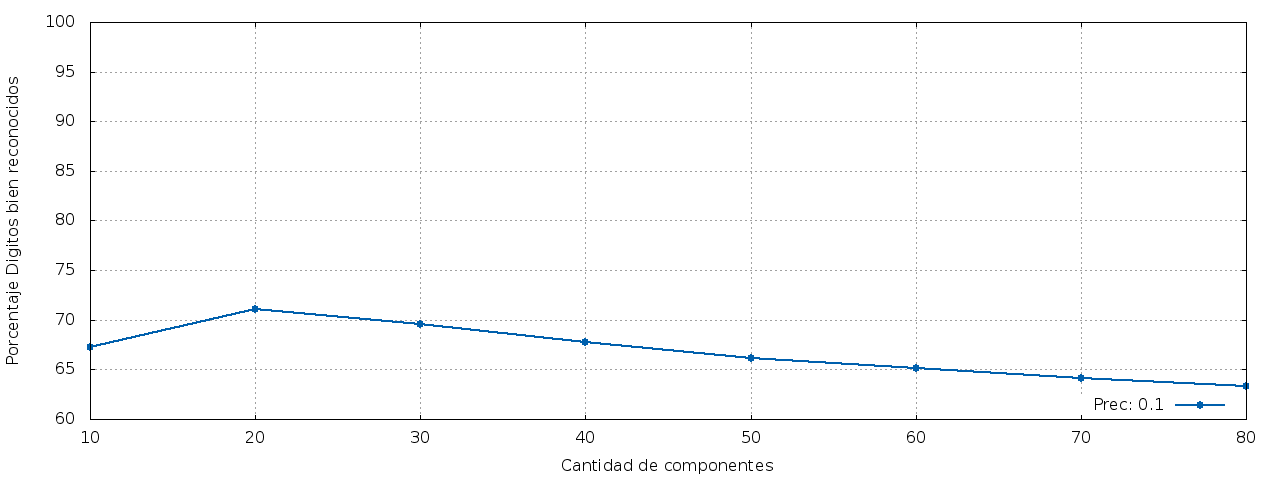
\includegraphics[width=20cm]{img/QRDistanciasMedias.png}}
		\centerline{\textsc{Cantidad de componentes Vs porcentaje de d\'igitos bien
		reconocidos}}
		\centerline{M\'etodo \textit{QR-potencia Inversa}/distancia al promedio en instancia \texttt{primeros5000.dat}}
		\vspace{5mm}


	\subsection{Influencia del tama\~no de la base de datos}

		Utilizando $5$ vecinos para el m\'etodo de los $k$-vecinos y una tolerancia
		de $0.001$ para los m\'etodos de reconocimiento de autovectores comparamos
		la cantidad de d\'igitos reconocidos usando un \textit{training set} de
		$6000$ im\'agenes y otro de $60000$ im\'agenes.
		La cantidad de componenes utilizada fue $50$ en el caso de los vecinos
		y $20$ en el caso de la distancia al promedio de las componentes.

		\vspace{5mm}
		\centerline{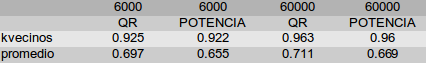
\includegraphics[width=12cm]{img/tamBaseDatos.png}}
		\centerline{\textsc{Porcentaje de d\'igitos bien reconocidos}}
		\centerline{\textsc{variando m\'etodos y tama\~no de \textit{training set}}}
		\centerline{Tolerancia $0.001$ en instancia \texttt{primeros5000.dat}}
		\vspace{5mm}


	\subsection{D\'igitos mejor reconocidos en funci\'on del m\'etodo}

		Comparamos \textit{hit rate} entre d\'igitos usando ambos metodos de reconocimiento
		de d\'igitos. Los autovectores se consiguen mediante el m\'etodo
		\textit{QR-potencia Inversa}\footnote{Ver Tabla F}:

		\vspace{5mm}
		\centerline{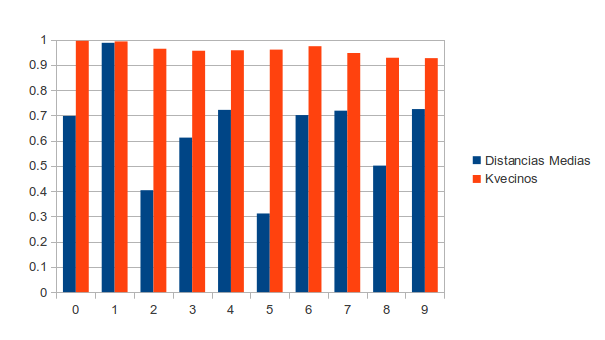
\includegraphics[width=14cm]{img/bam.png}}
		\centerline{\textsc{\textit{hit rate} de cada d\'igito}}
		\centerline{\textsc{variando m\'etodo de reconocimiento de d\'igitos}}
		\centerline{M\'etodo \textit{QR-potencia Inversa} con tolerancia $0.1$ en
		instancia \texttt{primeros5000.dat}}
		\vspace{5mm}
